\chapter{評価}
本章では,本研究で開発した個人認証システムの識別精度と登録及び認証処理にかかる時間の評価を行う.

% @suppress ParagraphNumber JapaneseAmbiguousNounConjunction InvalidSymbol
\section{識別精度の評価}
認証精度の評価について,端末を持ち上げるモーションを対象とする.
本システムを用いてあらかじめ6名の被験者に端末を持ち上げるモーションを4回入力してもらい,モーションデータの収集を行った.
各被験者ごとに,モーションデータの最初の3回分を登録モードにおける学習データ,最後の1回分を認証モードにおける入力データとして識別器の学習と識別を10回ずつ試行した.
また,それぞれの試行時になりすまし認証データとして筆者自身が同様のモーションを入力して得たモーションデータも入力した.

\begin{table}[btph]
  \centering
  \caption{識別精度の評価結果}
  \label{auth-result}
  \begin{tabular}{|c|r|r|r|r|r|} \hline
    回数 & 1 & 2 & 3 & 4 & 5 \\ \hline
    A & 0.438653 & 0.314004 & 0.331712 & 0.189229 & 0.343942 \\
    なりすまし & 0.999996 & 1 & 1 & 1 & 1 \\ \hline
    B & 0.643093 & 0.486959 & 0.30173 & 0.402533 & 0.333143 \\
    なりすまし & 0.92829 & 0.746492 & 0.471353 & 0.555157 & 0.990063 \\ \hline
    C & 0.463514 & 0.535742 & 0.429281 & 0.431916 & 0.660576 \\
    なりすまし & 0.511741 & 0.57337 & 0.585036 & 0.40849 & 0.897041 \\ \hline
    D & 0.542743 & 0.469785 & 0.478641 & 0.206191 & 0.316994 \\
    なりすまし & 0.51709 & 0.790494 & 0.860314 & 0.665402 & 0.366732 \\ \hline
    E & 0.369962 & 0.775177 & 0.930394 & 0.620721 & 0.861707 \\
    なりすまし & 0.425681 & 0.622781 & 0.823906 & 0.322503 & 0.808092 \\ \hline
    F & 0.427885 & 0.480025 & 0.526025 & 0.398201 & 0.602788 \\
    なりすまし & 0.440998 & 0.57856 & 0.40198 & 0.756612 & 0.580305 \\ \hline \hline
    回数 & 6 & 7 & 8 & 9 & 10 \\ \hline
    A & 0.451342 & 0.423822 & 0.25965 & 0.509021 & 0.202369 \\
    なりすまし & 1 & 1 & 1 & 1 & 0.997968 \\ \hline
    B & 0.335206 & 0.43043 & 0.403946 & 0.378164 & 0.412219 \\
    なりすまし & 0.605696 & 0.602051 & 0.312502 & 0.489541 & 0.951559 \\ \hline
    C & 0.416119 & 0.197132 & 0.515574 & 0.688828 & 0.635752 \\
    なりすまし & 0.612922 & 0.28289 & 0.712931 & 0.991952 & 0.580779 \\ \hline
    D & 0.403892 & 0.393019 & 0.457838 & 0.397036 & 0.63433 \\
    なりすまし & 0.677217 & 0.616272 & 0.60307 & 0.55076 & 0.533577 \\ \hline
    E & 0.558159 & 0.827285 & 0.816316 & 0.805877 & 0.741235 \\
    なりすまし & 0.457879 & 0.805894 & 0.486814 & 0.380957 & 0.529755 \\ \hline
    F & 0.403371 & 0.386153 & 0.492409 & 0.616016 & 0.389095 \\
    なりすまし & 0.430812 & 0.367287& 0.480061 & 0.511264 & 0.576477 \\ \hline
  \end{tabular}
\end{table}

この実験により識別器から得られた出力をまとめたものを表\ref{auth-result}に示す.
被験者Aと被験者Bについては本人のモーションデータから得られた出力が0に近く,なりすまし認証のモーションデータから得られた出力が1に近いことから良く識別できているといえる.
しかし他の4名の被験者について,なりすまし認証のモーションデータから得られた出力が本人のモーションデータから得られた出力より低く出ているものが多く,識別できていない結果となった.

本システムでは端末所有者のモーションデータとなりすまし認証によるモーションデータを識別するために,識別器の学習時に端末所有者のモーションデータのほかに,このデータと同じ値域で生成した乱数で一部を置き換えたダミーデータを用いた.
このダミーデータは元データの値域及び次元数に依存するため,端末所有者が入力したモーションが小さい場合は生成できる乱数の値域が限られることから,また次元数が少ない場合は置き換えるデータ数が少ないことから元データとの差があまり出ない可能性がある.
これにより,端末所有者が入力したモーションデータであってもなりすまし認証であると識別されてしまったのではないかと考えられる.

識別率の良かった被験者Aと良くなかった被験者Eのモーションデータを比較したものを図\ref{compare}に示す.

\begin{figure}[hbtp]
  \centering
  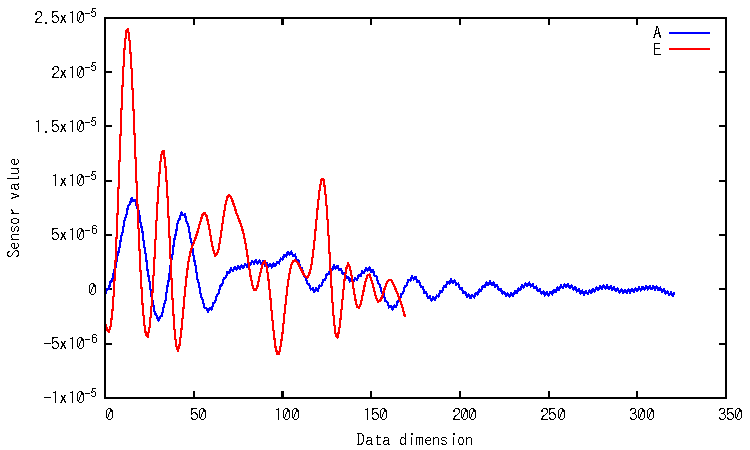
\includegraphics[bb=0 0 360 216, width=12cm]{Graphs/comp.pdf}
  \caption{被験者Aと被験者Eのモーションデータ比較}
  \label{compare}
\end{figure}

\section{登録及び認証の処理時間の評価}
本システムについて,登録及び認証の処理時間を計測した.
Androidのログ出力用APIとして用意されているLogクラス\cite{5-log}を用い,モーション入力が終了し計算処理中であることをユーザに示すプログレスダイアログが表示される部分と,登録及び認証処理が終わり処理結果が表示される前にプログレスダイアログが非表示となる部分にログ出力を行うコードを挿入した.
このログから出力される時刻情報から処理時間を求めて評価を行った.
また,認証モードについては端末内での計算処理も行えるため,こちらの処理時間も求めることとする.

評価の結果,サーバを用いた場合の登録処理ではおよそ65秒,認証処理ではおよそ2秒となった.
また,端末内での認証処理ではおよそ2.2秒となった.

ただし,モーションデータの次元数が多い場合や,サーバを多数のユーザが利用する場合はより長い処理時間を要すると考えられる.
